\section{Durchführung}
\label{sec:Durchführung}
Für den Versuch wird ein Drillachse wie in Abbildung \ref{fig:Drillachse} verwendet.
\begin{figure}
  \centering
  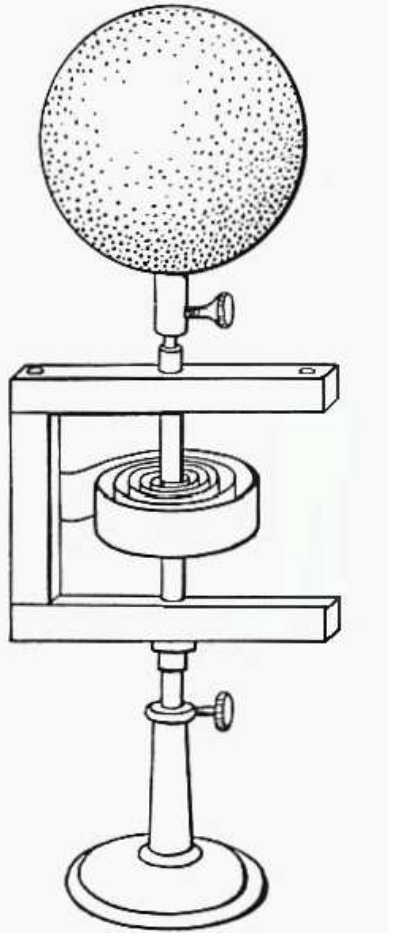
\includegraphics[width=0.14\textwidth]{Drillachse.png}
  \caption{Abbildung der Messapparatur \cite{sample}.}
  \label{fig:Drillachse}
\end{figure}
Die Apparaturkonstanten die Winkelrichtgrößen $D$ und das Trägheitsmoment $I_D$ werden bestimmt.
Dafür wird die Drillachse in einem Abstand $r$ in eine Federwaage eingehängt, um den Winkel $\phi$
ausgelenkt und mit Gleichung \eqref{eqn:Winkelrichtgroesse} die Winkelrichtgröße bestimmt.
Um das Trägheitsmoment $I_D$ zu bestimmen wird an der Drillachse eine möglichst masselosen Stange
mit zwei gewichten  senkrecht zur Drehachse befestigt. Das system wird in Schwingung
versetzt und die Schwingungsdauer $T$ gemessen. Die Schwingungsdauern werden quadratisch
zu den Abstandsquadraten aufgetragen, und dann wird das Eigenträgheitsmoment mittel
linearer Regression und Gleichung \eqref{eqn:Periodetorrosion} bestimmt.
Als nächstes werden die Trägheitsmomente von zwei verschiedenen Körpern durch
Gleichung \eqref{eqn:Periodetorrosion} bestimmt werden. dafür werden die Körper auf der Drillachse
befestigt, das System in Schwingung versetzt und die Schwingungsdauer Gemessen.
Nun wird nach der Selben Methode das Trägheitsmoment einer Puppe in zwei verschiedenen
Haltungen gemessen. Um die Ergebnisse zu vergleichen verden die Formen der Körper
und Puppen vermessen und ihr Gewicht bestimmt. Bei der Puppe werden dafür die Körperteile
Kopf, Beine, Arme und Rumpf als Zylinder genähert.
